\documentclass[../main.tex]{subfiles}

\begin{document}

\section{Definitions}
\begin{itemize}
  \item Generative models: any model that takes in a training set, samples drawn from distribution $p_{data}$ and learns to represent an estimate of that distribution somehow, the result is a distribution $p_{model}$
\end{itemize}


\section{Generative Adversarial Networks}
\subsection{Why GANs?}
\begin{itemize}
  \item High-dimensional probability distributions are important
  \item Can be incorporated into reinforcement learning:
  \begin{itemize}
    \item simulate possible futures by learning a conditional distribution over future states
    \item enable learning in an imaginary environment
    \item guide exploration by keeping tracking of how often different states have been visited
    \item inverse reinforcement learning
  \end{itemize}
  \item Provide predictions on inputs that are missing data (e.g. semi-supervised learning)
  \item Enable machine leanring to work with multi-modal outputs
  \item Many tasks require realistic generation of samples from some distributions
  \begin{itemize}
    \item Single image super-resolution
    \item Creating art
    \item Image-to-image translation
  \end{itemize}

  \item
  \begin{figure}[h]
    \caption{Taxonomy of deep generative models}
    \centering
    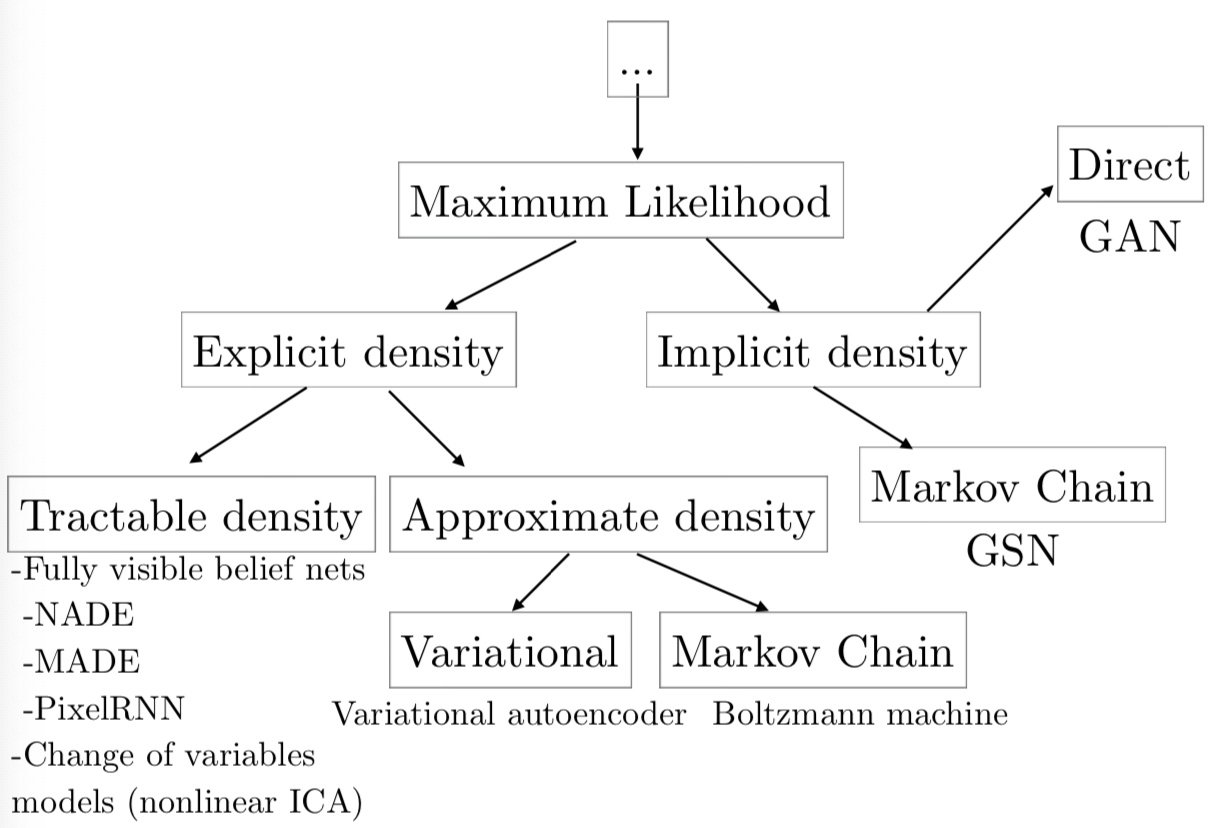
\includegraphics[width=0.5\textwidth]{../imgs/generative_models.png}
  \end{figure}

  \item Benefits
  \begin{itemize}
    \item Can generate samples in parallel
    \item Design of generator has few restrictions
    \item No Markov Chains are needed
    \item No variational bound is needed
    \item Produces better samples than other methods
  \end{itemize}

\end{itemize}

\subsection{How do GANs work?}
\begin{itemize}
  \item Game between two players: the generator and the discriminator
  \item Generator $(G)$
  \begin{itemize}
    \item creates samples that are intended to come from the same distribution as the training data
    \item typically implemented as a deep neural network
    \item inputs $z$ are sampled from a prior over latent variables and generator $G(z)$ creates a new fake sample
    \item different formulations of loss function
    \begin{enumerate}
      \item minimax, zero sum game
      \item $J^{(G)} = - J^{(D)}$
      \item amenable to theoretical analysis
      \item heuristic
      \item maximum-likelihood game
    \end{enumerate}

  \end{itemize}
  \item Discriminator $(D)$
  \begin{itemize}
    \item examines samples to determine whether they are real or fake
    \item output probability that input sample $x$ is real
    \item goal is for $D(x)$ to be near 1
    \item also wanted to make $D(G(z))$ approach 0
    \item cost function:
    \begin{equation*}
      J^{(D)}(\theta^{(D)}, \theta^{(G)}) = -\frac{1}{2} \mbb{E}_{x \sim p_{data}} [log(D(x))] - \frac{1}{2} \mbb{E}_{z} [log(1- D(G(z)))]
    \end{equation*}
    \item this is the cross entropy loss, pretty standard across all discriminator loss functions
    \item classifier is trained on two minibatches of data: one from the dataset (label = 1) and another from the generator (label = 0)
  \end{itemize}
  \item The solution to a game is the Nash equilibrium

  \item tmp
 \end{itemize}


\end{document}